\documentclass[tikz]{standalone}
\usetikzlibrary{arrows,automata}
\usepackage[utf8]{inputenc}
\begin{document}
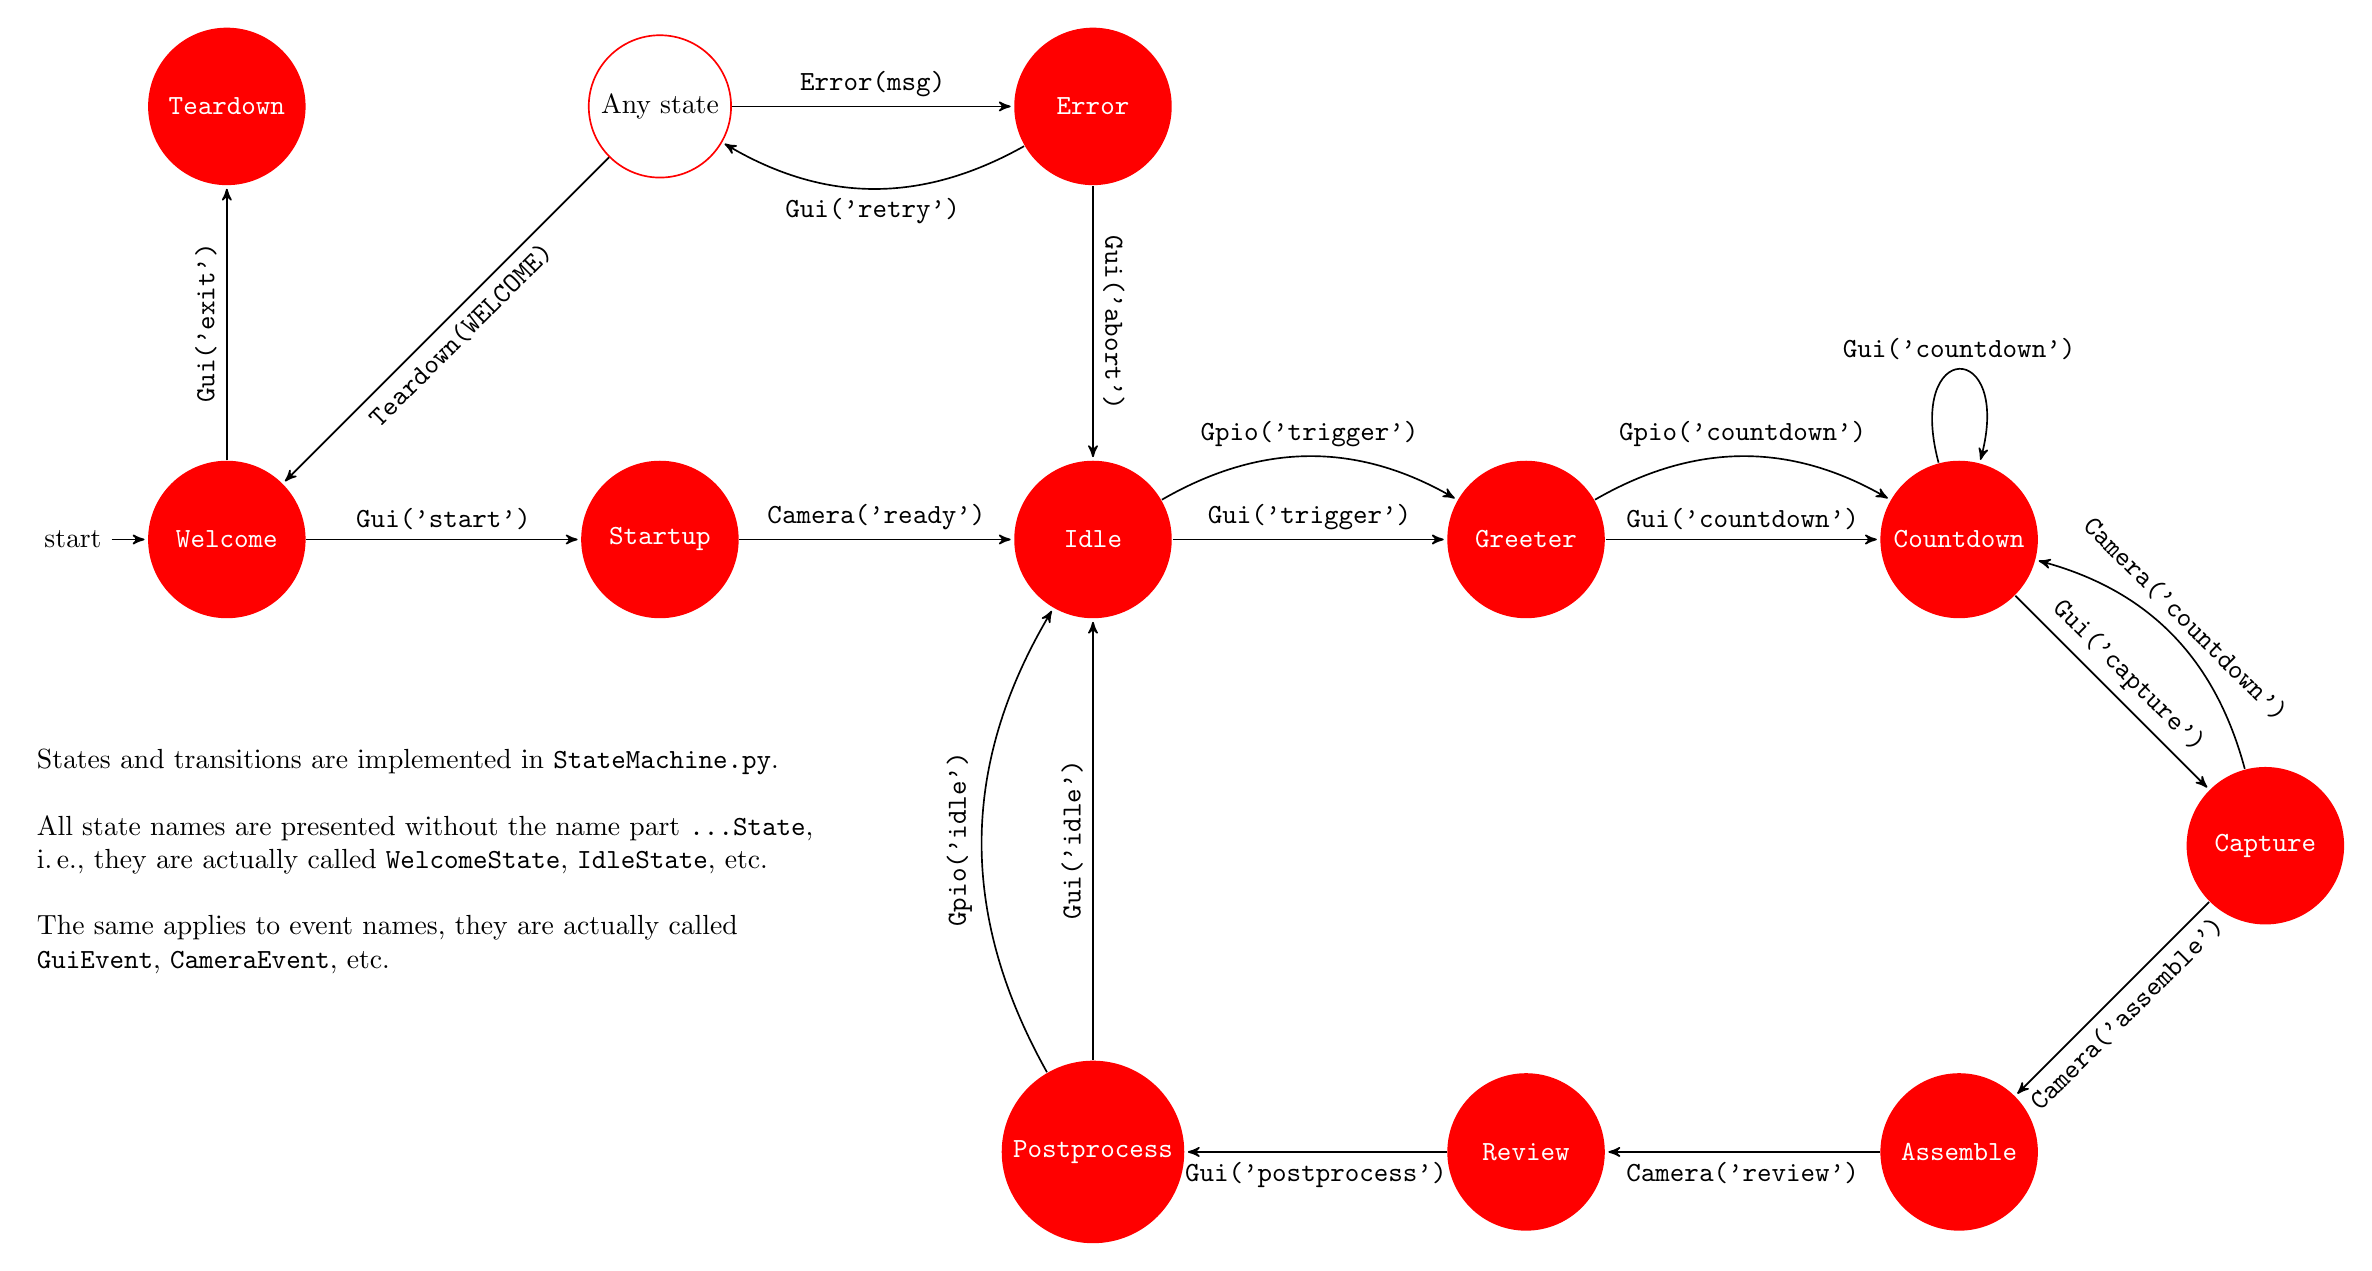
\begin{tikzpicture}[->,>=stealth',shorten >=1pt,auto,node distance=5.5cm,
                    semithick]
  \tikzstyle{every state}=[fill=red,draw=none,text=white,minimum width=2cm]

  \node[initial,state]  (Welcome)                             {\texttt{Welcome}};
  \node[state]          (Startup)   [right of=Welcome]        {\texttt{Startup}};
  \node[state]          (Teardown)  [above of=Welcome]        {\texttt{Teardown}};
  \node[state]          (Idle)      [right of=Startup]        {\texttt{Idle}};
  \node[state]          (Greeter)   [right of=Idle]           {\texttt{Greeter}};
  \node[state]          (Countdown) [right of=Greeter]        {\texttt{Countdown}};
  \node[state]          (Capture)   [below right of=Countdown]{\texttt{Capture}};
  \node[state]          (Assemble)  [below left of=Capture]   {\texttt{Assemble}};
  \node[state]          (Review)    [left of=Assemble]        {\texttt{Review}};
  \node[state]          (Postprocess) [left of=Review]        {\texttt{Postprocess}};

  \node[state]          (Error)     [above of=Idle]           {\texttt{Error}};
  \node[circle,draw,red,text=black] (Any) [left of=Error]    {Any state};

  \path (Welcome)   edge              node {\texttt{Gui('start')}} (Startup)
        (Welcome)   edge              node [rotate=90,anchor=south] {\texttt{Gui('exit')}}  (Teardown)
        (Startup)   edge              node {\texttt{Camera('ready')}} (Idle)
        (Idle)      edge              node {\texttt{Gui('trigger')}} (Greeter)
        (Idle)      edge [bend left]  node {\texttt{Gpio('trigger')}} (Greeter)
        (Greeter)   edge              node {\texttt{Gui('countdown')}} (Countdown)
        (Greeter)   edge [bend left]  node {\texttt{Gpio('countdown')}} (Countdown)
        (Countdown) edge [loop above] node {\texttt{Gui('countdown')}} (Countdown)
        (Countdown) edge              node [rotate=-45,anchor=south] {\texttt{Gui('capture')}} (Capture)
        (Capture)   edge [bend right] node [rotate=-45,anchor=south] {\texttt{Camera('countdown')}} (Countdown)
        (Capture)   edge              node [rotate=45,anchor=north] {\texttt{Camera('assemble')}} (Assemble)
        (Assemble)  edge              node {\texttt{Camera('review')}} (Review)
        (Review)    edge              node {\texttt{Gui('postprocess')}} (Postprocess)
        (Postprocess) edge            node [rotate=90,anchor=south] {\texttt{Gui('idle')}} (Idle)
        (Postprocess) edge [bend left] node [rotate=90,anchor=south] {\texttt{Gpio('idle')}} (Idle)
        (Any)       edge              node {\texttt{Error(msg)}} (Error)
        (Error)     edge              node [rotate=-90,anchor=south] {\texttt{Gui('abort')}} (Idle)
        (Error)     edge [bend left]  node {\texttt{Gui('retry')}} (Any)
        (Any)       edge              node [rotate=45,anchor=north] {\texttt{Teardown(WELCOME)}} (Welcome);

  \node [text width=10cm,anchor=north west] at (current page.south west) 
  {
    States and transitions are implemented in \texttt{StateMachine.py}. \\[1.2em]
    All state names are presented without the name part \texttt{...State}, i.\,e., they are actually called \texttt{WelcomeState}, \texttt{IdleState}, etc. \\[1.2em]
    The same applies to event names, they are actually called \texttt{GuiEvent}, \texttt{CameraEvent}, etc.
  };
\end{tikzpicture}
\end{document}